\documentclass{article}
\usepackage[utf8]{vietnam}
\usepackage{graphicx} % Required for inserting images
\usepackage{placeins}
\usepackage[english]{babel}
\usepackage{array} % For better column formatting
% Set page size and margins
% Replace `letterpaper' with `a4paper' for UK/EU standard size
\usepackage[letterpaper,top=2cm,bottom=2cm,left=3cm,right=3cm,marginparwidth=1.75cm]{geometry}

% Useful packages
\usepackage{amsmath}
\usepackage{graphicx}
\usepackage[colorlinks=true, allcolors=blue]{hyperref}

\title{Multi-icon from Multi-Label Text Classification}
\author{
Pham Tran Tuan Khang\\
Quach Tuan Anh\\
Dinh Van Kien\\
Nguyen Tran Nghia
}
\date{Hanoi, December 2024}


\begin{document}
\maketitle
\begin{abstract}
Multi-label text classification is a critical task in natural language processing (NLP) that involves assigning multiple relevant labels to a single textual input. This project proposes a novel approach to infer multiple policies or categories from text and map these multi-label outputs to interactive multi-icon representations for enhanced user engagement. Using a BERT-based deep learning model, the system is fine-tuned on the Reuters-21578 dataset for general topic classification and further refined using the GoEmotions dataset to incorporate emotion-specific policy inference. The proposed model is evaluated using standard metrics such as Hamming Loss, F1 Score, Precision, and Recall, with k-fold cross-validation ensuring robust performance assessment. The results demonstrate significant improvements over the baseline models such as logistic regression and random forests. The introduction of multi-icon mapping provides a visually intuitive and interactive way to represent complex multilabel outputs, making the system applicable to policy analysis, content moderation, and other domains requiring efficient text categorization. Future work will explore scalability, integration with additional datasets, and enhanced visualization techniques.
\end{abstract}

\tableofcontents
\section*{Project Team Roles}
\begin{table}[h!]
    \centering
    \renewcommand{\arraystretch}{1.3} % Adjust row height
    \begin{tabular}{| m{5cm} | m{5cm} | m{7cm} |}
        \hline
        \textbf{Member Name} & \textbf{Responsibilities} \\ 
        \hline
        Pham Tran Tuan Khang  & Exploratory Data Analysis \\ & Model evaluation \\ & Models serving/deployment \\ 
        \hline
        Quach Tuan Anh & Data preprocessing \\ & Model development \\
        \hline
        Dinh Van Kien & Data preprocessing  \\ & Model development \\ 
        \hline
        Nguyen Tran Nghia & Exploratory Data Analysis \\ & Researching \\ & Documentation \\
        \hline
    \end{tabular}
    \caption{Roles and Responsibilities of Project Members}
    \label{tab:team_roles}
\end{table}
\section{Introduction}
\subsection{Overview of the project}
The increasing volume of unstructured text data in various domains has created a demand for automated systems capable of efficiently categorizing and analyzing content. Multi-label text classification, which assigns multiple relevant labels to a single input, plays a crucial role in addressing this challenge. This project proposes the development of a deep learning-based system that not only performs multi-label classification but also translates the results into interactive multi-icon representations. By leveraging pre-trained language models such as BERT, the system aims to infer multiple relevant policies or categories from textual input, providing both accurate categorization and an engaging user experience through visual representations. The integration of multi-icon mapping enhances the interpretability of the model outputs, making the results more accessible and intuitive.
\subsection{Problem statement}
Manual text categorization is time-consuming and error-prone, especially when dealing with multi-label classification tasks where a single text can belong to multiple categories. Existing solutions often struggle with overlapping labels, ambiguity in text, and scalability to large datasets. Furthermore, traditional approaches lack user-friendly ways to present multi-label outputs, which limits their utility in real-world applications like policy inference or sentiment analysis. This project addresses these challenges by developing a BERT-based model fine-tuned on diverse datasets (Reuters-21578 for topic classification and GoEmotions for emotion-specific categorization). Additionally, it introduces a novel multi-icon mapping system, which converts multi-label outputs into visually interactive icons, improving the usability and interpretability of the results.
\subsection{Significance of the project}
This project is significant for several reasons:

- Automating Policy Inference: The proposed system automates the process of identifying relevant policies or categories from text, which is particularly useful in domains such as policy analysis, legal document classification, and content moderation.

- Improved User Interaction: By mapping multi-label outputs to multi-icons, the project enhances the way information is presented, making it more intuitive and engaging for end users. This can benefit applications requiring quick decision-making or visual summaries of complex data.

- Advancing Multi-Label Classification: Leveraging state-of-the-art deep learning models such as BERT, this work contributes to advancements in multi-label text classification by addressing challenges like label overlap, scalability, and emotion-specific inference.

- Cross-Domain Applicability: The inclusion of datasets like Reuters-21578 and GoEmotions ensures that the model is adaptable to various domains, from news categorization to emotion-driven policy recommendations.

By combining cutting-edge NLP techniques with interactive visualization, this project provides a novel solution that bridges the gap between accurate text classification and user-centric design.
\section{Problem definition}
\subsection{Problem definition}
The task of multi-label text classification involves assigning multiple relevant categories or labels to a single input text. This is particularly challenging due to the following reasons:

- Overlapping Labels: Many real-world datasets, including those used in this project, exhibit overlapping labels where a single text can belong to multiple categories. For instance, a news article may simultaneously fall under "Economy" and "Politics."

- Ambiguous and Diverse Text Inputs: Text data often contains ambiguity, domain-specific language, or emotions, which makes it harder for traditional models to capture the nuances required for accurate classification.

- Scalability: With large datasets like Reuters-21578, which contains 90 topics, the task becomes computationally expensive, and it is essential to use models that can generalize well without overfitting.

- Presentation of Results: While most classification systems output textual labels, they often fail to present the results in a user-friendly and visually interpretable way. This limits their usability for stakeholders who prefer more interactive or visual representations.

To address these challenges, this project proposes a BERT-based model designed for multi-label classification, fine-tuned on topic and emotion datasets, and introduces a novel multi-icon mapping system to enhance the interpretability and usability of the results. The system aims to provide accurate policy or category inference while also addressing the need for engaging and intuitive visualization.
\subsection{Base Knowledge of Sentiment Analysis}
Sentiment analysis, or opinion mining, is a key area of natural language processing (NLP) that determines the emotional tone of text, categorizing it as positive, negative, or neutral. Advanced techniques can identify nuanced emotions like joy, anger, or despair. The three main approaches to sentiment analysis are lexicon-based methods, machine learning, and deep learning. Lexicon-based methods rely on predefined word dictionaries, while machine learning uses algorithms like Naïve Bayes, SVM, and Logistic Regression to learn from labeled data. Deep learning models, including RNNs, LSTMs, and transformers like BERT, excel at capturing context for superior performance.

Implementing sentiment analysis involves preprocessing (e.g., text cleaning, tokenization, embedding generation), model training, and evaluation using metrics like accuracy and F1-score. Tools such as scikit-learn, TensorFlow, and Hugging Face Transformers streamline development. Applications range from monitoring social media trends to analyzing customer feedback and survey data, providing valuable insights into public opinion and emotional responses.

In our project, sentiment analysis improves the accuracy of emoji predictions by practicing BERT’s ability to capture emotional and contextual nuances. The preprocessing steps, including text cleaning and tokenization, feed into the model training on curated datasets. This integration ensures that emoji recommendations align with the text sentiment, creating more intuitive and relatable outputs. Sentiment analysis thus forms the foundation for mapping textual emotions to meaningful multiicon representations, finalizing with the output is rewritten version of original text with more interactive icon.
\section{Dataset}
The project utilizes two datasets, each serving a distinct purpose in the model's development and evaluation:
\subsection{Reuters-21578}
Reuters-21578 is a seminal dataset in text classification, originally compiled by Reuters news agency. The dataset contains approximately 21,578 news articles spanning around 135 unique categories, primarily focused on business, financial, and general news reporting from the late 1980s. As a benchmark in multi-label document categorization, it provides researchers with a rich collection of English-language texts that require sophisticated classification techniques.

The dataset's significance lies in its complex nature, where each document can be associated with multiple categories simultaneously. This characteristic makes it an exceptional resource for developing advanced machine learning models that can navigate the nuanced landscape of document classification. Researchers have long valued Reuters-21578 for its diversity of topics, which range from corporate news to global economic trends, making it an ideal playground for testing and refining multi-label classification algorithms.

\subsection{GoEmotions}
GoEmotions represents a more contemporary approach to text classification, developed by researchers at Google using over 58,000 Reddit comments. This dataset stands out for its focus on emotion detection, featuring 27 distinct emotional categories derived from user-generated social media content. By capturing the intricate emotional landscape of online communication, GoEmotions provides a unique lens into the complexity of human emotional expression through text.

The dataset's manual verification process ensures high-quality ground truth annotations, making it particularly valuable for developing sophisticated emotion recognition models. Emotions range from subtle states like admiration and gratitude to more intense feelings such as anger and excitement. The multi-label nature of the dataset reflects the real-world complexity of emotional communication, where individuals often experience and express multiple emotions simultaneously.

These datasets offer complementary approaches to text classification. Reuters-21578 provides a structured, professional perspective on multi-label categorization, while GoEmotions captures the more nuanced, personal dimensions of emotional communication. For research focused on developing advanced multi-label inference models, these datasets present an opportunity to explore the intricate ways text can be classified across different domains and emotional spectrums.
\subsection{Exploratory Data Analysis}
We visualized several charts to facilitate the analysis of the dataset prior to training our models. These charts are provided in Appendix \ref{sec:EDA_charts}. In this section, we will discuss the key characteristics identified for each dataset and outline our data preprocessing strategy to ensure proper compatibility with our deep neural network models.

For Reuters dataset, the largest category is "earn" with over 3,400 documents, followed by "acq" with around 2,300 documents. Several other notable categories include "money-fx", "grain", "crude", and "trade". This indicates the dataset has a diverse set of topics, with a clear skew towards economic and financial themes. The"earn" is the dominant category at 39.7\%, with "acq" as the second largest at 23.7\%. This aligns with the bar chart, showing the strong representation of these two categories compared to the others. The next tier includes "money-fx", "grain", and "crude" which each make up 4-7\% of the dataset. Shifting to document characteristics, the dataset has a mixture of very short (1-2 word) documents as well as some much longer outliers. The majority of documents appear to be quite concise, with a steep drop-off in frequency as document length increases. There was the vast differences in representation, with "earn" being the clear standout at over 3,500 occurrences. Many other categories have frequencies below 100, indicating they are much more sparsely populated in the dataset.Overall, Reuters is heavily skewed towards economic and financial topics, with a "earn" and "acq" dominating the category distribution. The document lengths also suggest a mix of very concise and more verbose content. 

For GoEmotion dataset, the majority of records (36,308) have 1 class assigned to them. There are significantly fewer records with 2, 3, 4, and 5 classes, with the counts dropping off sharply as the number of classes increases. This indicates that the dataset is primarily single-labeled, with most texts belonging to a single emotion category. The most prevalent emotion is 'neutral' with over 14,219 occurrences, followed by 'sadness' at around 4,130 occurrences. Other notable emotions include 'fear', 'disgust', 'anger', and 'anticipation'. The chart shows a wide range in the representation of different emotions, with some being much more common than others. This dataset show the high frequency of texts of the length 200. However, the distribution also shows a long tail, with some texts being significantly longer. This suggests the dataset contains a mix of short and long texts, with the majority being of moderate length.

Overall, the Reuters-21578 dataset appears to be heavily skewed towards economic and financial topics, with the "earn" and "acq" categories dominating the distribution. In contrast, the GoEmotion dataset focuses on emotion-based classification, with a wide range of emotion categories represented, though "neutral" is the most prevalent. In terms of the number of classes per record, the Reuters-21578 dataset seems to have a more diverse set of multilabel assignments, with a significant number of documents having 2, 3, or more categories. The GoEmotion dataset, on the other hand, is primarily single-labeled, with the vast majority of texts belonging to only one emotion class. Regarding the text length distributions, both datasets exhibit a mix of shorter and longer documents. The Reuters-21578 dataset appears to have a more even spread, while the GoEmotion dataset shows a clear spike around 200 characters, suggesting a preference for moderately-sized texts. The differences in the focus and characteristics of these two datasets make them suitable for complementary use cases in multilabel sentiment analysis on social media posts. The Reuters-21578 dataset could be valuable for tasks involving financial or economic sentiment analysis, where identifying multiple relevant topics is important. The GoEmotion dataset, on the other hand, would be well-suited for fine-grained emotion detection and analysis of social media content, capitalizing on its robust representation of various emotion categories.By utilizing both datasets in a multilabel sentiment analysis framework, researchers and practitioners can gain a more comprehensive understanding of the sentiment and emotions expressed in social media posts. The Reuters-21578 dataset can provide insights into the broader thematic context, while the GoEmotion dataset can offer detailed emotional nuances. This combined approach can lead to more accurate and meaningful sentiment analysis, enabling better understanding of user sentiment and engagement on social media platforms.

In summary, the Reuters-21578 and GoEmotion datasets, with their distinct characteristics and focus areas, can be valuable resources for conducting multilabel sentiment analysis on social media posts. Leveraging the strengths of both datasets can lead to more robust and insightful sentiment analysis models, ultimately driving better decision-making and customer engagement strategies in various domains.

\subsection{Data preprocessing}
To prepare the datasets for training, several preprocessing steps were performed to ensure data quality and compatibility with the BERT-based model. First, text cleaning was conducted by removing unnecessary characters, punctuation, and special symbols. Additionally, all text was converted to lowercase to maintain uniformity across the dataset. Following this, tokenization was applied using BERT's tokenizer, which splits the text into tokens while preserving contextual information essential for the model.

Next, stopword removal was performed to eliminate common words such as "the" and "and" that do not add significant meaning, thereby reducing noise and focusing on meaningful content. To address the issue of imbalanced labels, techniques such as oversampling or weighted loss functions were implemented, particularly for categories with fewer occurrences, to ensure that the model did not overlook these minority labels.

The datasets were then split into training, validation, and test sets using a standard 70-20-10 ratio to enable robust evaluation and prevent overfitting during training. Labels were transformed into a binary matrix format through multi-label encoding, where each row represents a text and columns indicate the presence or absence of specific categories. Lastly, sequence padding was applied to ensure that all input sequences had a uniform length. Shorter texts were padded, and longer texts were truncated as required by the input specifications of the BERT model.

These preprocessing steps collectively ensured that the datasets were clean, balanced, and structured appropriately for effective training and evaluation, optimizing both the efficiency and performance of the classification model.

\section{Model Architecture}
\subsection{First approach: Simple Deep Neural Network}

\subsubsection{Model Architecture, Loss Function, Optimizer, and Optimization Parameters}
\begin{figure}[h!]
  \centering
  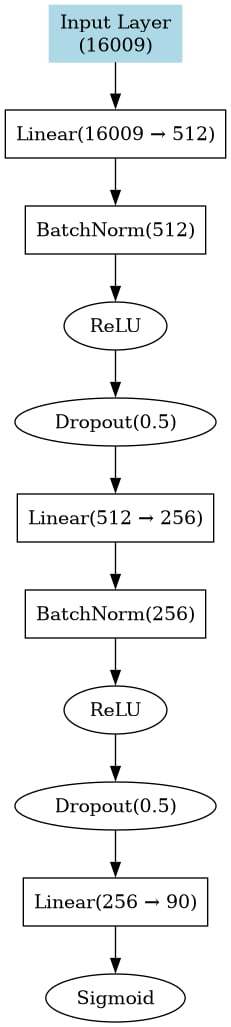
\includegraphics[width=0.2\textwidth]{DNN.png} 
  \caption{Illustration of overall structure of the model.}
  \label{fig:your-label}
\end{figure}
We first practice a simple deep neural network architecture for this problem, as shown in Appendix .Its comprises several sequential linear transformations, interspersed with non-linear activation functions, batch normalization, and dropout layers. The initial layer is a linear layer transforming the input from a dimensionality of $n_{in}$, corresponding to the size of the TF-IDF vocabulary, to a hidden layer of 512 nodes. This linear transformation is followed by batch normalization, a technique that normalizes the layer's activations across each mini-batch, stabilizing training and enabling the use of larger learning rates. A ReLU (Rectified Linear Unit) activation function is subsequently applied, introducing non-linearity crucial for the model to learn complex patterns in the data. To prevent overfitting, a dropout layer is applied after the ReLU layer with a rate of 0.5, which randomly deactivates 50\% of the neurons during training. This process of linear transformation, batch normalization, ReLU activation, and dropout is repeated, reducing the dimensionality of the hidden layer to 256. Finally, the output layer is a linear layer that projects the representation to $n_{out}$ nodes, corresponding to the number of classes present in the multi-label problem. This is followed by a sigmoid activation function on each of the output nodes, which squashes the output to a range between 0 and 1, allowing multi-label classification of each output independently. Sigmoid is the right choice for multi-label text classification because it models the probability of each label independently, allowing the model to predict multiple labels simultaneously. Softmax is designed for multi-class classification, where only one label can be present at a time.


For optimization, the model uses a Binary Cross-Entropy (BCE) loss function. BCE is suitable for multi-label problems where each label is treated as an independent binary classification. The loss quantifies the divergence between the predicted probabilities and true labels. This loss is minimized by the model using the Adam optimizer, a variant of gradient descent that dynamically adapts the learning rate of each parameter, typically leading to faster and more effective convergence. The learning rate is initialized at 0.001. Further, the training uses the ReduceLROnPlateau learning rate scheduler. This adaptive scheduler monitors the training loss. If the loss plateaus (does not improve) for 3 epochs (patience=3), the scheduler reduces the learning rate by a factor of 0.1, to make sure the model is able to fine-tune better as the training process goes. The model is optimized by adjusting weights and biases through backpropagation, which uses the gradients of the loss function with respect to model's parameters. 

The training loss used as the primary metric for optimization in this model because of its direct relationship with the loss function and gradient. It’s used to optimize the model’s internal parameters through gradient descent. While validation metrics (such as F1 or validation loss) are crucial for model selection, performance assessment, and hyperparameter tuning, they aren’t suitable for the gradient-based optimization process, since their gradients are not used to update model's parameters. So, using training loss to directly optimize model parameters ensures that we are addressing the fundamental goal of learning to make accurate predictions. 

\subsubsection{Data Flow Operation and Iterations}
The training process begins with data preparation, where the text data is transformed into TF-IDF feature vectors and the labels are encoded using the MultiLabelBinarizer. These are then converted to PyTorch tensors, which are packaged into TensorDataset objects, and finally, loaded by PyTorch's DataLoader, which creates mini-batches for the optimization process. Each training epoch then proceeds in the following manner: the model is set to training mode (model.train()), enabling dropout and batch normalization. For each mini-batch of training data, the following operations are done:


The mini-batch is transferred to the specified device. The gradients of the model parameters are reset by calling \texttt{optimizer.zero\_grad()} to ensure that the gradients are computed for the current batch of samples. Then, the training input data \texttt{batch\_x} is passed through the model through \texttt{output=model(batch\_x)} to obtain the predicted probability of each output class, which is a forward pass through the network. The output is then compared to the true labels using the Binary Cross Entropy loss function by \texttt{loss = self.criterion(outputs, batch\_y)}. The backpropagation is done via \texttt{loss.backward()}, which calculates the gradients with respect to the model parameters. The optimizer updates model parameters according to the gradients computed in the previous step by \texttt{optimizer.step()}. This process updates the model’s weights, moving it towards minimizing the training loss. The training loss calculated in the forward pass is also accumulated to be used to monitor the training progress and trigger the learning rate scheduler.

After each epoch, the training set performance is evaluated using model.evaluate(), with dropout deactivated through \texttt{model.eval()}, and accuracy, f1, precision and recall are computed and reported for analysis. During the whole training process, the model with the best training loss is saved. Once the training is complete, the model with the best training loss is loaded, and the model performance is then evaluated on a test set to provide a comprehensive performance report on a previously unseen dataset.
\subsection{Recurrent Neural Network with Long Short-Term Memory (LSTM)}
\subsubsection{Model Architecture, Loss Function, Optimizer, and Optimization Parameters}

\begin{figure}[h!]
  \centering
  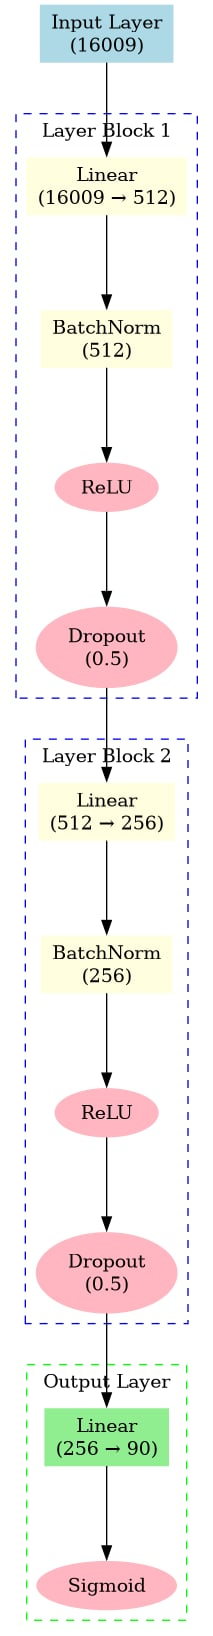
\includegraphics[width=0.1\textwidth]{LSTM.png} 
  \caption{Illustration of overall structure of the model.}
  \label{fig:your-label}
\end{figure}

The implemented model, LSTMClassifier, is designed for multi-label text classification, utilizing a Long Short-Term Memory (LSTM) network at its core. The input to the model consists of sequences of feature vectors, usually derived from TF-IDF representations of text. These vectors are treated as sequences of length one using an unsqueeze operation, but in a real setting they might represent sequence of words of input texts. The model's first and most critical component is a bidirectional LSTM layer. LSTMs, a form of recurrent neural network, are chosen for their capacity to process sequential data and learn dependencies across time steps through their internal cell state. This particular LSTM layer is bidirectional, meaning it processes the input sequence both forwards and backwards, allowing it to capture contextual information from both past and future sequence positions, using bidirectional=True. The LSTM layer is configured with specific parameters: \texttt{input\_size}, which is the dimensionality of each input feature vector; \texttt{hidden\_size} of 256, defining the capacity of the LSTM; \texttt{num\_layers} of 2, allowing for deeper learning of more complex dependencies; \texttt{batch\_first=True}, dictating the input data format; and dropout regularization with a rate of 0.5, applied if the number of LSTM layers is greater than 1, to combat overfitting and vanishing gradient problems.

Following the LSTM layer, the outputs, which are the concatenated hidden states from both forward and backward passes, are fed into a series of linear and batch normalization layers. Because of the bidirectionality of the LSTM (Which can help model captures context from both past and future directions), the output's dimension is \texttt{2 * hidden\_size}. These linear layers serve to transform the complex, sequential representation from the LSTM into a format suitable for multi-label classification. The first linear layer reduces the dimensionality from the concatenated LSTM output \texttt{(2 * hidden\_size)} to 512. Batch normalization, ReLU activation, and dropout regularization follows this layer. This pattern is then repeated with a second linear layer which further transforms and reduces the dimensionality of the data to 256, followed by the same batch norm, ReLU and dropout layers. Finally, the model culminates in a linear output layer that maps the transformed features to \texttt{n\_out} nodes, corresponding to the number of classes in the multi-label classification task. This output layer is then activated by a sigmoid function, which outputs independent probabilities between 0 and 1 for each class, enabling the model to make predictions regarding the presence of multiple classes simultaneously. 


The Binary Cross-Entropy (BCE) loss function is employed to quantify the divergence between the predicted probabilities and the true labels, and the model's parameters are updated by Adam optimizer, with ReduceLROnPlateau learning rate scheduler to allow adaptive learning rate and better fine-tuning as training proceeds.The training loss was chosen to be the primary optimization metric due to its direct relationship with the loss function and gradients.
\subsubsection{Data Flow, Iterations, and Training Process (LSTM)}
The training process begins with the preparation of the data using \texttt{prepare\_data}. Input features and labels, in the form of TF-IDF vectors and multi-label encodings respectively, are transformed into PyTorch tensors. These are then bundled into TensorDataset objects and loaded into DataLoader instances, which handle batching and shuffling for training efficiency. The \texttt{train\_epoch} method executes one training epoch as follows: first, the model is set to training mode to enable dropout and batch normalization layers, and all gradients are reset by \texttt{optimizer.zero\_grad()}. For each batch, the input data is moved to the appropriate device (CPU or GPU) and passed through the model during the forward pass, calculating the predicted probabilities for each class. The predicted probabilities are then compared to the true labels, and the BCE loss is calculated, which represents the divergence between the model's predictions and the actual labels. Backpropagation is then performed to calculate the gradients of the loss function with respect to the model parameters. The optimizer then updates the model parameters based on these gradients in an attempt to reduce the training loss. The average training loss is accumulated and returned.

During evaluation, the model is set to evaluation mode with \texttt{model.eval()}, which disables dropout and batch normalization layers, ensuring deterministic performance. The evaluate method iterates through the batches of the evaluation dataset and calculates metrics such as loss, accuracy, F1-score, precision, and recall. The predicted probabilities are then thresholded to decide if the class is predicted to be present or not. During the whole training process, the model with the best training loss is saved. This model is loaded once training is completed and then evaluated on a test set to provide the final assessment of its generalization capabilities using the same evaluation method. The overall training process is managed by the \texttt{train\_model} function. This function iterates through the training data for a fixed number of epochs, and reports the training metrics for each epoch. The ReduceLROnPlateau scheduler is also used to adjust learning rate during training, with learning rate reduction if the training loss stops improving. The training process is designed to minimize the training loss, improve the generalization capability of the model, and provides feedback to the user about the model performance during the training process.
\subsection{Attention based Graph Neural Network}
When dealing with the problem of Multi-label Text Classification (MLTC), the dependency structures among labels has proven to be a crucial yet challenging aspect to capture effectively. For this second approach, we implemented a multi-head attention mechanism to extract the correlation between labels for MLTC task.

\subsubsection{Model Architecture}
The model has two main components that work in parallel. On the text processing side, input text is first embedded using BERT and then processed through a BiLSTM network to generate feature vectors that capture the textual content. On the graph side, the model represents labels as nodes in a graph, where each node's features are the label embeddings, and the connections between nodes are represented by a learnable adjacency matrix that captures label correlations.
\begin{figure}[h!]
  \centering
  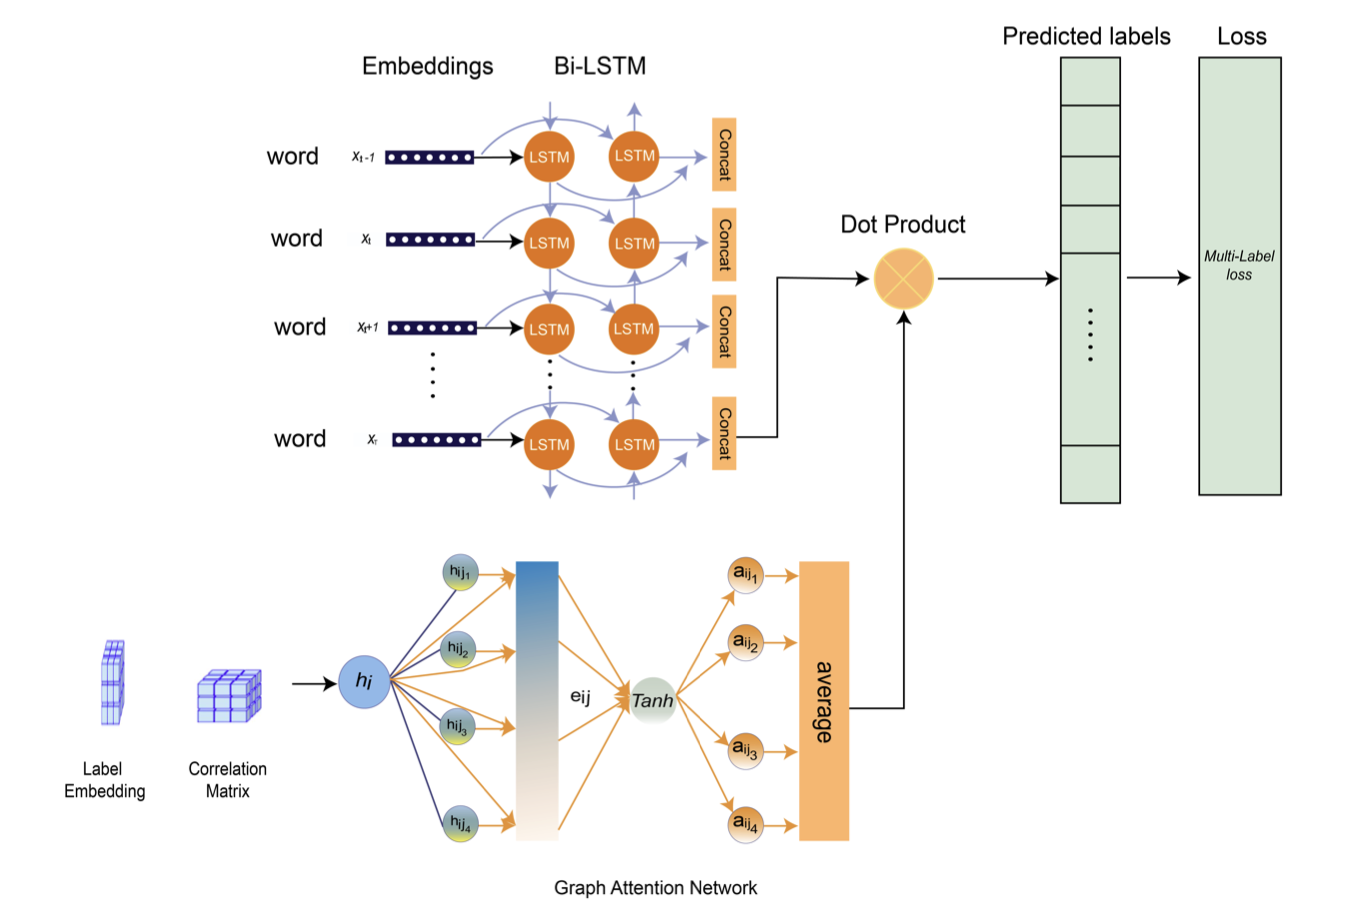
\includegraphics[width=\textwidth]{Magnet.png} 
  \caption{Illustration of overall structure of the model.}
  \label{fig:your-label}
\end{figure}
This graph structure is processed through Graph Attention Network (GAT) layers that use multi-head attention mechanisms to learn the importance of relationships between different labels. The GAT layers produce attended label features by aggregating information from neighboring nodes weighted by learned attention coefficients. In the final step, the model combines the BiLSTM's text feature vectors with the attended label features through multiplication to generate the final prediction scores. The adjacency matrix can be initialized in three ways: as an identity matrix, using Xavier initialization, or using a correlation matrix based on label co-occurrences in the training data. The entire model is trained end-to-end using cross-entropy loss.
\subsubsection{Graph representation of labels}
In our approach, we represent the label relationships as a graph structure $G$, where we have a feature matrix $M \in \mathbb{R}^{n\times d}$ and an adjacency matrix $A \in \mathbb{R}^{n\times n}$. Here, $n$ represents the total number of possible labels, and $d$ is the feature dimensionality.

Unlike traditional graph-based approaches where the graph structure is predefined, our model learns the adjacency matrix dynamically. This learned structure enables the model to discover and represent complex relationships between labels. The key innovation lies in treating label embeddings as node features while maintaining a trainable adjacency matrix that adapts during the learning process.

\subsubsection{Node updating Mechanism in Graph convolution}
The fundamental operation in our graph convolutional architecture involves updating node representations through neighborhood aggregation. For any node $i$ at layer $\ell$, the update follows:

\begin{equation}
H^{(\ell+1)} = \sigma\left(AH^{(\ell)}W^{(\ell)}\right)
\end{equation}

This mechanism enables information flow between connected labels, allowing the model to capture label dependencies.

\subsubsection{Graph Attention Networks for multi-label classification}
To enhance the model's ability to capture varying importance of label relationships, we implement an attention mechanism. This replaces the uniform weighting of standard GCNs with learned attention weights. The attention-based update for a node becomes:

\begin{equation}
H_2^{(\ell+1)} = \text{ReLU}\left(\alpha_{22}^{(\ell)}H_2^{(\ell)}W^{(\ell)} + \alpha_{21}^{(\ell)}H_1^{(\ell)}W^{(\ell)} + \alpha_{23}^{(\ell)}H_3^{(\ell)}W^{(\ell)} + \alpha_{24}^{(\ell)}H_4^{(\ell)}W^{(\ell)}\right)
\end{equation}

The attention coefficients are computed using:

\begin{equation}
\alpha_{ij}^{(\ell)} = f\left(H_i^{(\ell)}W^{(\ell)}, H_j^{(\ell)}W^{(\ell)}\right)
\end{equation}

\begin{equation}
\alpha_{ij} = \text{ReLU}\left((H_iW) \parallel (H_jW)^T\right)
\end{equation}

We employ multi-head attention to stabilize learning:

\begin{equation}
H_i^{(\ell+1)} = \text{Tanh}\left(\frac{1}{K}\sum_{k=1}^K\sum_{j\in N(i)}\alpha_{ij,k}^{(\ell)}H_j^{(\ell)}W^{(\ell)}\right)
\end{equation}

\subsubsection{Feature vector generation}
Our text encoding pipeline combines BERT embeddings with a bidirectional LSTM architecture. The BiLSTM processes the sequence in both directions:

\begin{align}
\vec{h}_i &= \overrightarrow{\text{LSTM}}(\vec{h}_{i-1}, x_i) \\
\overleftarrow{h}_i &= \overleftarrow{\text{LSTM}}(\overleftarrow{h}_{i+1}, x_i)
\end{align}

The complete representation combines both directions:
\begin{equation}
h_i = [\vec{h}_i; \overleftarrow{h}_i]
\end{equation}

The final feature vector is computed as:
\begin{equation}
F = f_{rnn}(f_{BERT}(s; \theta_{BERT}); \theta_{rnn}) \in \mathbb{R}^D
\end{equation}

The prediction is generated through:
\begin{equation}
\hat{y} = F \odot H_{gat}
\end{equation}

\subsubsection{Adjacency matrix generation}
We explore three distinct initialization strategies for the adjacency matrix:

\begin{itemize}
\item A basic identity matrix initialization
\item Xavier initialization with bounds:
\begin{equation}
\pm\sqrt{\frac{6}{n_i + n_{i+1}}}
\end{equation}
\item A correlation-based initialization:
\begin{equation}
A = M / F
\end{equation}
\end{itemize}

\subsubsection{Loss function}
The model is trained using binary cross-entropy loss for multi-label classification:

\begin{equation}
L = \sum_{c=1}^C y_c\log(\sigma(\hat{y}_c)) + (1-y_c)\log(1-\sigma(\hat{y}_c))
\end{equation}

This loss function effectively handles the multi-label nature of our classification task, where each input can belong to multiple classes simultaneously.
\section{Evaluation}
\subsection{Training process}
\subsubsection{Deep Neural Network}
\begin{figure}[h!]
  \centering
  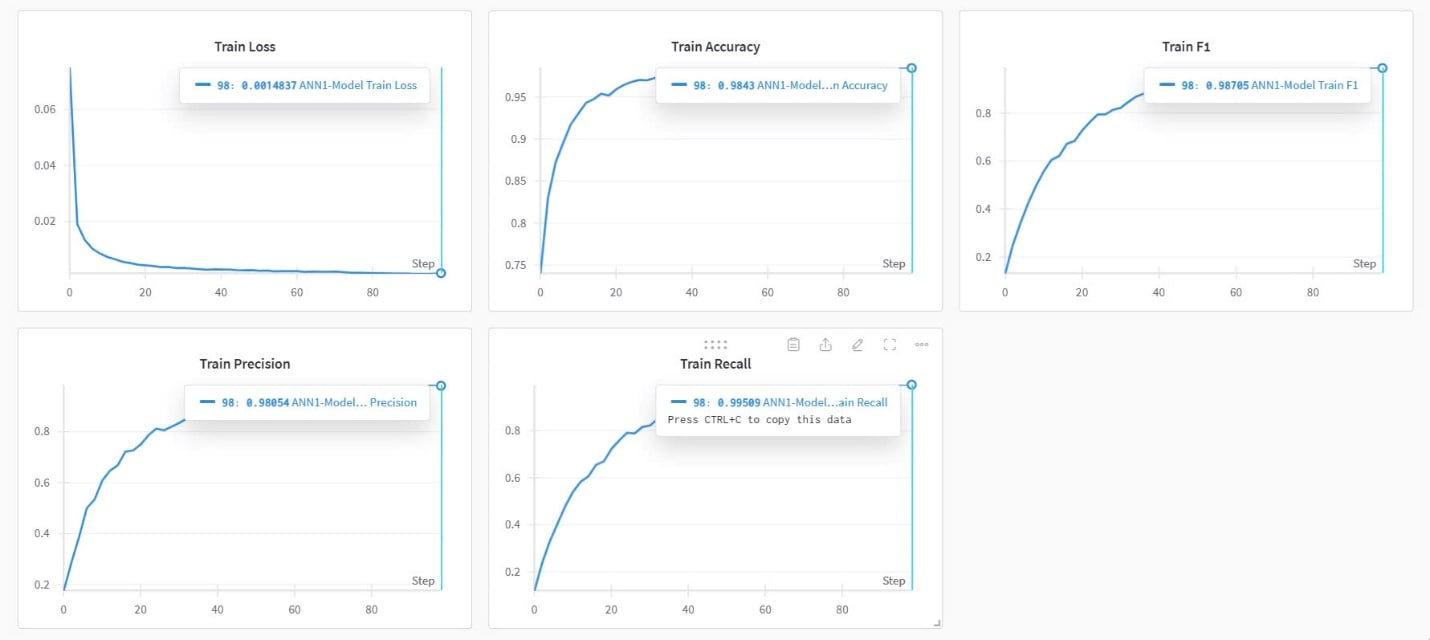
\includegraphics[width=\textwidth]{DNN_TRAIN.jpeg} 
  \caption{Evaluation Metrics for first approach on training set.}
  \label{fig:your-label}
\end{figure}
\begin{figure}[h!]
  \centering
  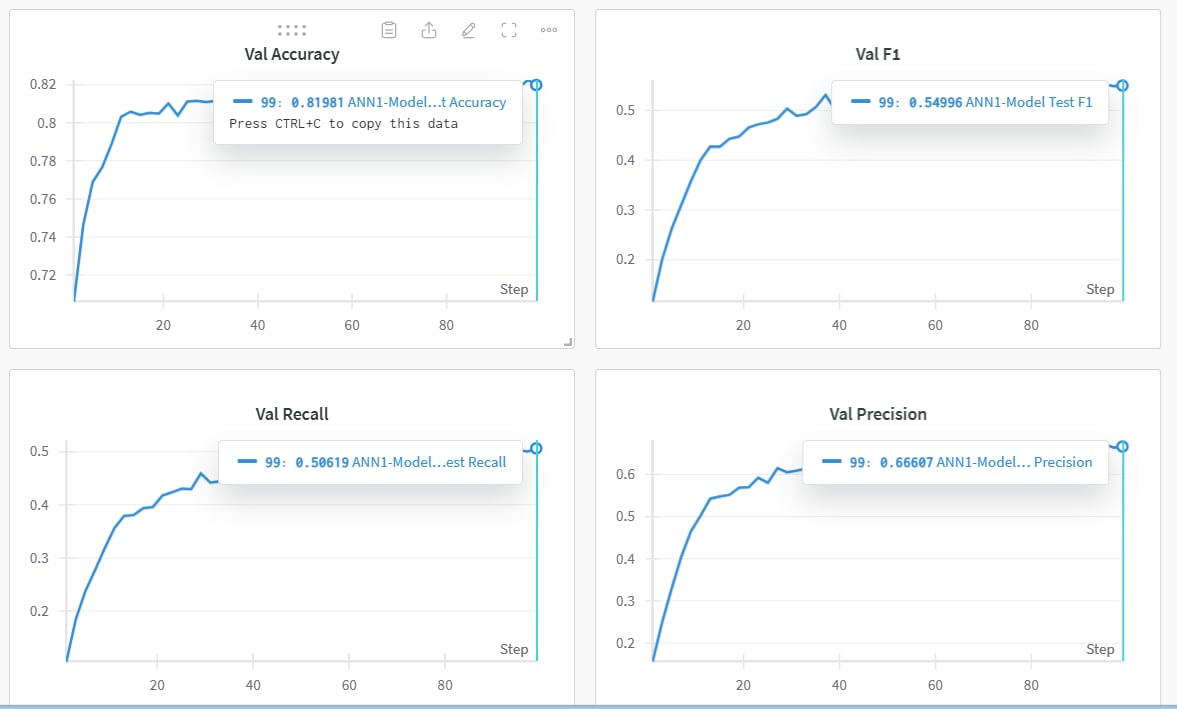
\includegraphics[width=\textwidth]{DNN_VAL.jpeg} 
  \caption{Evaluation Metrics for first approach on cross-validation set.}
  \label{fig:your-label}
\end{figure}

\FloatBarrier

\subsubsection{LSTM}
\begin{figure}[h!]
  \centering
  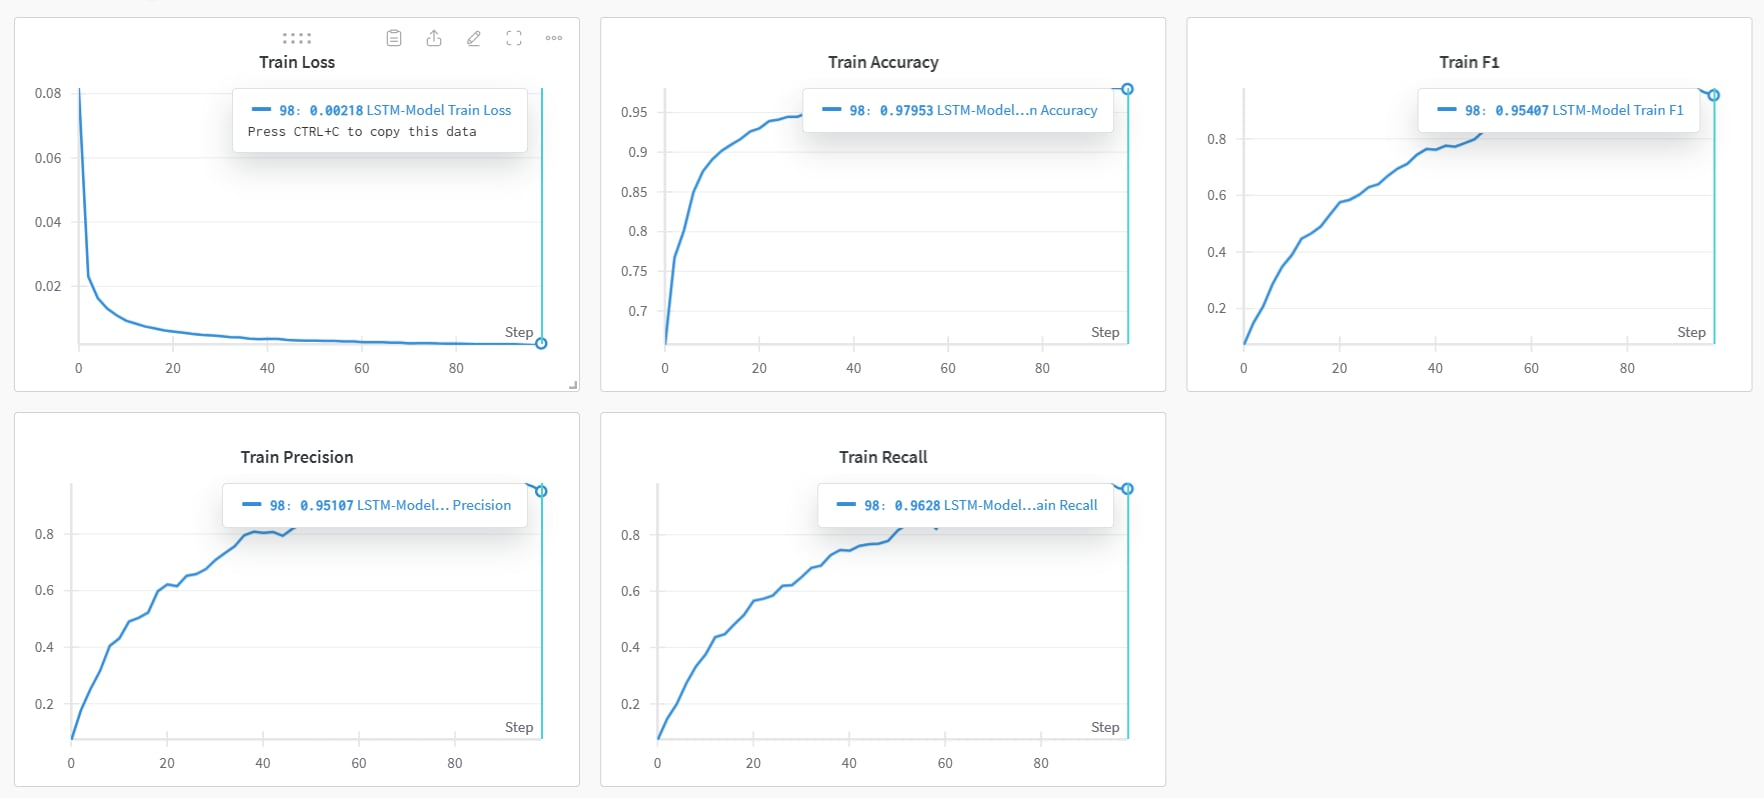
\includegraphics[width=\textwidth]{LSTM_TRAIN.jpeg} 
  \caption{Evaluation Metrics for second approach on training set.}
  \label{fig:your-label}
\end{figure}
\begin{figure}[h!]
  \centering
  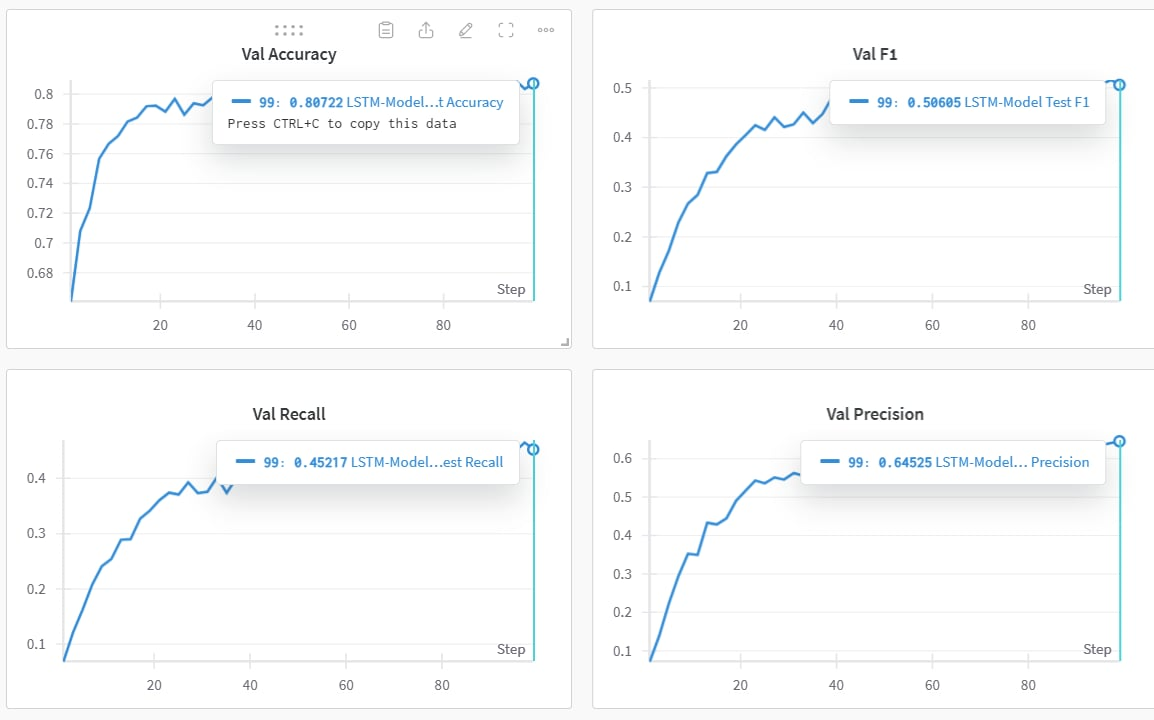
\includegraphics[width=\textwidth]{LSTM_VAL.jpeg} 
  \caption{Evaluation Metrics for second approach on cross-validation set.}
  \label{fig:your-label}
\end{figure}

\FloatBarrier
\subsubsection{Magnet (TA Viet)} 
\begin{figure}[h!]
  \centering
  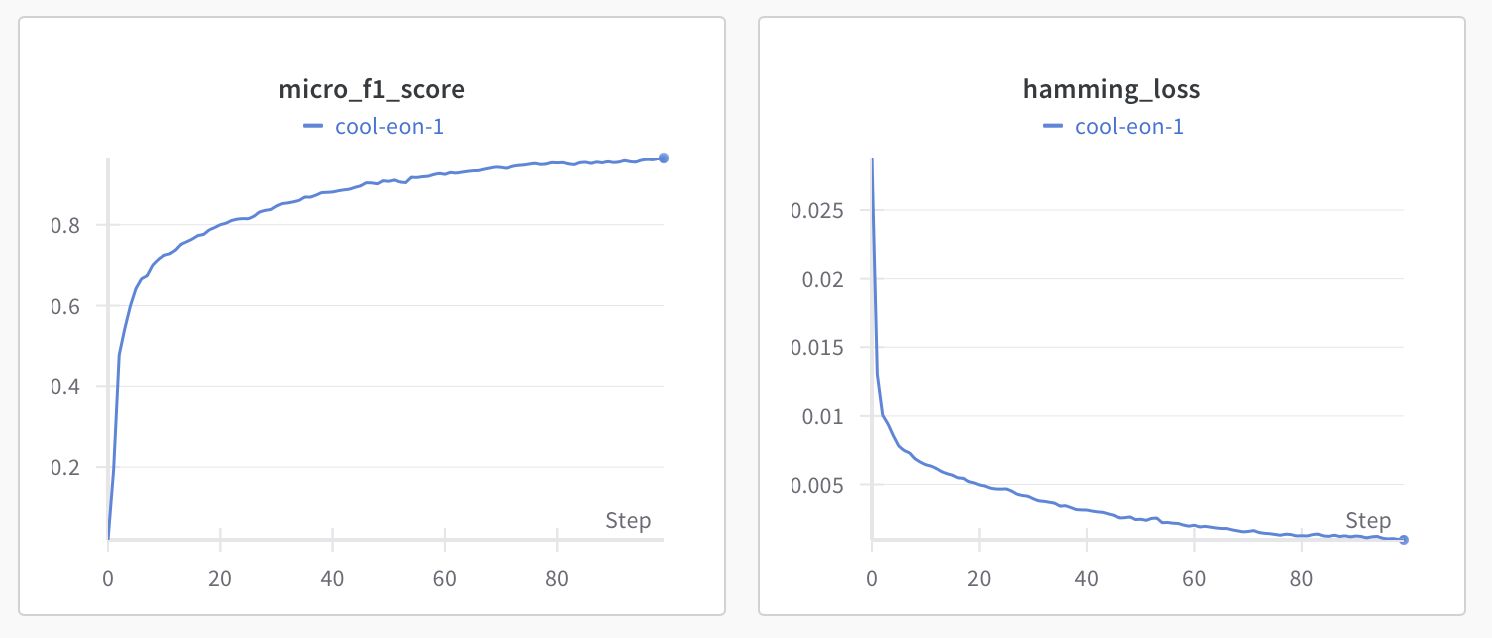
\includegraphics[width=\textwidth]{magnet_f1.png} 
  \caption{Evaluation Metrics for third approach on test set.}
  \label{fig:your-label}
\end{figure}
\subsection{Performace on Test-set}
These are performace of models on each dataset for our defined accurracy metric
\begin{table}[h!]

    \centering
    \begin{tabular}{l|c|c}
         \textbf{Model} & \textbf{Reuters (\%)} & \textbf{GoEmotion \%)} \\
         \hline
         DNN  & 84.2 & 66.6 \\
         LSTM  & 84.6 & 71.5 \\
         MAGNET  & 85.7 & 77.2 \\
         % YOLO v5 & 89.6 & 86.9 \\
    \end{tabular}
    \caption{Model Performance on Accuracy} 
    \label{tab:model_performance_comparison}
\end{table}

\begin{table}[h!]
    \centering
    \begin{tabular}{l|c|c}
         \textbf{Model} & \textbf{Reuters (\%)} & \textbf{GoEmotion \%)} \\
         \hline
         DNN (Kien) & 50.6 & 63.5 \\
         LSTM (Kien) & 78.1 & 69.3 \\
         MAGNET (Tuan Anh) & 83.3 & 55.3 \\
         % YOLO v5 & 89.6 & 86.9 \\
    \end{tabular}
    \caption{Model Performance on F1 score } 
    \label{tab:model_performance_comparison}
\end{table}

\begin{table}[h!]
    \centering
    \begin{tabular}{l|c|c}
         \textbf{Model} & \textbf{Reuters (\%)} & \textbf{GoEmotion \%)} \\
         \hline
         DNN & 45.4 & 61.8 \\
         LSTM & 77.3 & 70.1 \\
         MAGNET & 89.2 & 62.2 \\
         % YOLO v5 & 89.6 & 86.9 \\
    \end{tabular}
    \caption{Model Performance for Recall} 
    \label{tab:model_performance_comparison}
\end{table}

\begin{table}[h!]
    \centering
    \begin{tabular}{l|c|c}
         \textbf{Model} & \textbf{Reuters (\%)} & \textbf{GoEmotion \%)} \\
         \hline
         DNN  & 64.5 & 65.5 \\
         LSTM  & 80.1 & 67.5 \\
         MAGNET  & 86.0 & 68.2 \\
         % YOLO v5 & 89.6 & 86.9 \\
    \end{tabular}
    \caption{Model Performance for Precision.} 
    \label{tab:model_performance_comparison}
\end{table}
\FloatBarrier
Based on the performance analysis of the three models (DNN, LSTM, and MAGNET) across two datasets (Reuters and GoEmotion), MAGNET consistently outperforms the other models in most metrics for both datasets. For accuracy, MAGNET achieves the highest performance on both Reuters (85.7\%) and GoEmotion (77.2\%), highlighting its robustness in general classification tasks. In terms of F1 score, MAGNET excels on Reuters (83.3\%) but shows a lower performance on GoEmotion (55.3\%), indicating that while it performs well on balanced datasets like Reuters, it may struggle with more nuanced datasets like GoEmotion. The recall metric further emphasizes MAGNET's strength in detecting relevant features from Reuters (89.2\%), but it performs comparably to DNN and LSTM on GoEmotion, achieving 62.2\%. For precision, MAGNET again achieves the highest score on Reuters (86.0\%) and maintains a competitive performance on GoEmotion (68.2\%).

While MAGNET demonstrates superior performance on Reuters across all metrics, the results on GoEmotion suggest that its strength may be dataset-dependent. LSTM performs well overall, particularly on GoEmotion, where it achieves competitive accuracy (71.5\%), F1 score (69.3\%), recall (77.3\%), and precision (80.1\%), indicating its ability to handle complex emotional content better than DNN and MAGNET in certain cases. DNN, on the other hand, consistently underperforms in comparison to the other models, particularly on Reuters, where it achieves the lowest scores across all metrics. This highlights the limitations of simpler models like DNN in handling complex datasets. Overall, MAGNET is the most robust model, but LSTM shows promise in handling datasets with emotional content.
\section{Models deployment}
We developed a Gradio interface where the input is a text segment, and the output is the same text enhanced with sentiment-based icons, as shown in appendix \ref{sec:demo_ui}. Using the sentiment produced by our deep neural network models for each segment of the sentence, we map the sentiment labels generated by the model to corresponding icons. These icons are then embedded into appropriate places in the sentence, making it more interactive and visually engaging.

The potential applications of this tool are wide-ranging. It can be used in social media platforms to enhance user posts by adding relevant emojis, effectively increasing engagement and making the content more relatable. In customer feedback analysis, this tool can visually highlight sentiment trends in reviews or surveys, enabling businesses to identify issues and patterns quickly. It can also enrich content personalization by adding emojis to emails, chat messages, or notifications, improving user experience by making communication more empathetic.

In education, the tool can help students or writers better understand the tone and sentiment in texts, while in mental health analysis, it can aid in detecting emotional states in written content, providing counselors or therapists with valuable insights. Additionally, the tool can improve team communication by clarifying the tone of messages in internal chats, reducing misunderstandings. It can also be integrated into chatbots and AI assistants to make responses more engaging and empathetic.

Furthermore, the tool has applications in marketing and advertising, where sentiment-based emojis can enhance ad copy by evoking the desired emotions and grabbing attention. It can also assist in summarizing long-form content by visually representing emotional highlights, allowing readers to quickly understand key takeaways. Lastly, it can be used in interactive storytelling, enhancing the narrative by visually representing characters' emotions with emojis. Overall, this tool has immense potential to improve communication and emotional clarity across a variety of domains.

\section{Reference}
\begin{thebibliography}{99}
\bibitem{Pal_2020}
Pal, A., Selvakumar, M., and Sankarasubbu, M. (2020).
\textit{MAGNET: Multi-Label Text Classification using Attention-based Graph Neural Network}.
In \textit{Proceedings of the 12th International Conference on Agents and Artificial Intelligence}, pages 494-505. SCITEPRESS - Science and Technology Publications.

\bibitem{vennerød2021longshorttermmemoryrnn}
Vennerød, C. B., Kjærran, A., and Bugge, E. S. (2021). Long Short-term Memory RNN. \emph{arXiv preprint arXiv:2105.06756}.
\bibitem{demszky2020goemotionsdatasetfinegrainedemotions}
Demszky, D., Movshovitz-Attias, D., Ko, J., Cowen, A., Nemade, G., and Ravi, S. (2020). GoEmotions: A Dataset of Fine-Grained Emotions. \emph{arXiv preprint arXiv:2005.00547}.
\bibitem{devlin2019bertpretrainingdeepbidirectional}
Devlin, J., Chang, M., Lee, K., and Toutanova, K. (2019). BERT: Pre-training of Deep Bidirectional Transformers for Language Understanding. \emph{arXiv preprint arXiv:1810.04805}.
\bibitem{Pal_2020}
Pal, A., Selvakumar, M., and Sankarasubbu, M. (2020). MAGNET: Multi-Label Text Classification using Attention-based Graph Neural Network. In \emph{Proceedings of the 12th International Conference on Agents and Artificial Intelligence}, pages 494-505. SCITEPRESS - Science and Technology Publications.
\end{thebibliography}
\appendix
\section{Exploratory Data Analysis charts}\label{sec:EDA_charts}
\begin{figure}[h!]
  \centering
  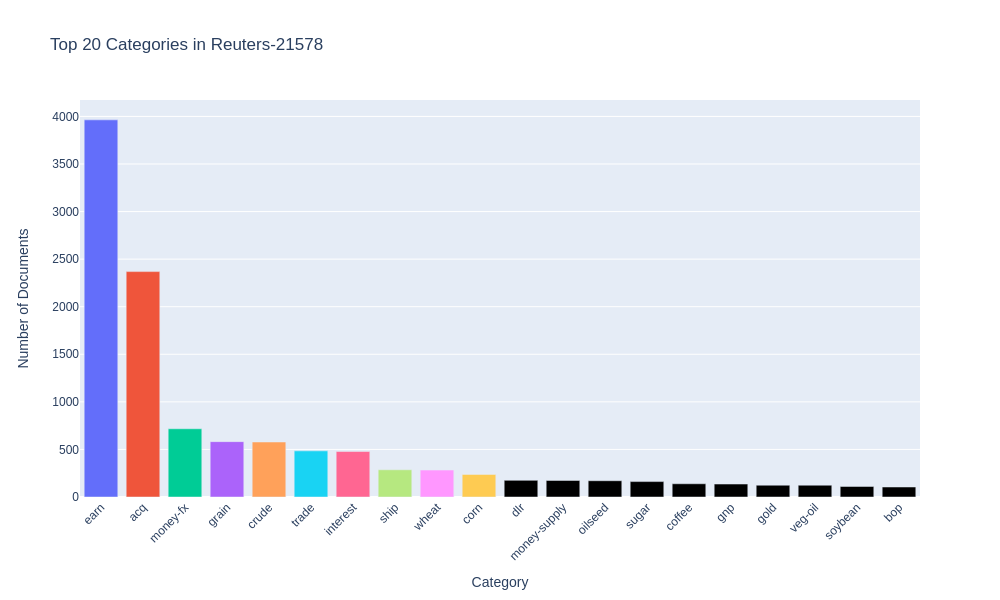
\includegraphics[width=1\textwidth]{reuter1.png} 
  \caption{Caption for your image}
  \label{fig:your-label}
\end{figure}
\begin{figure}[h!]
  \centering
  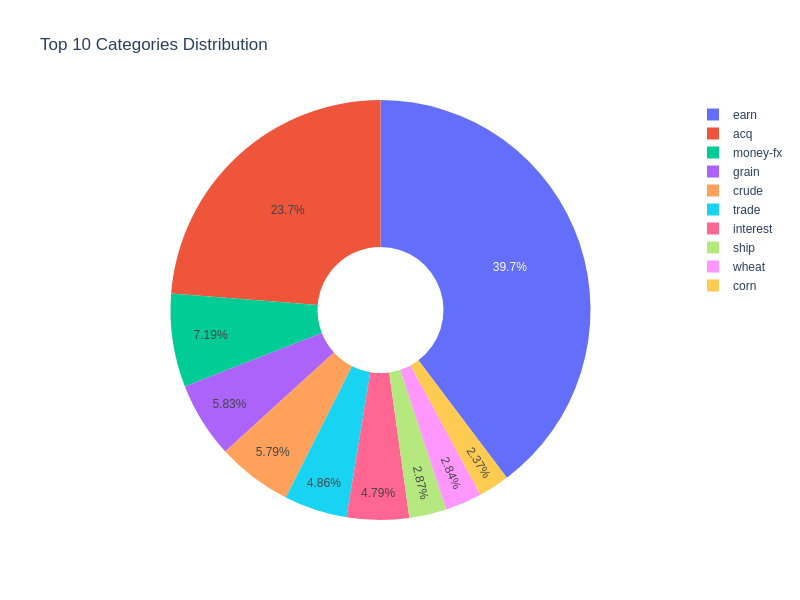
\includegraphics[width=1\textwidth]{reuter2.png} 
  \caption{Caption for your image}
  \label{fig:your-label}
\end{figure}
\begin{figure}[h!]
  \centering
  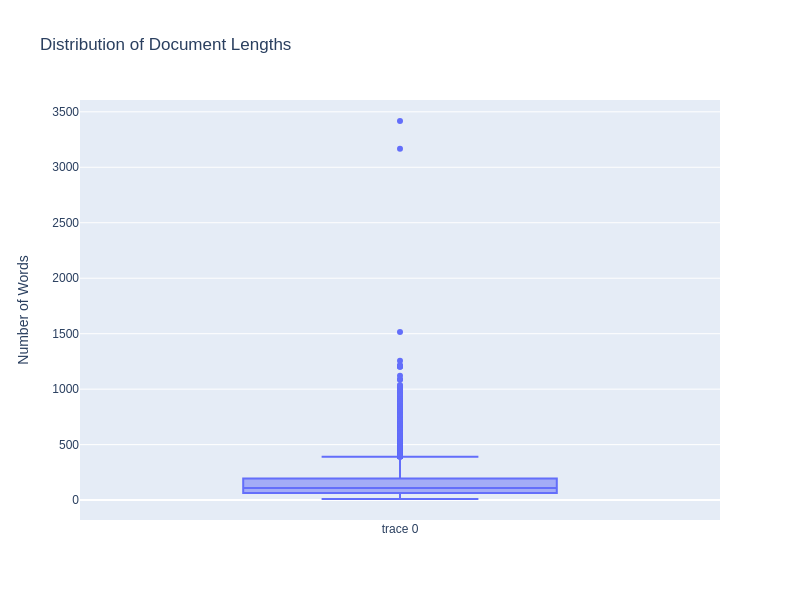
\includegraphics[width=1\textwidth]{reuter3.png} 
  \caption{Caption for your image}
  \label{fig:your-label}
\end{figure}
\begin{figure}[h!]
  \centering
  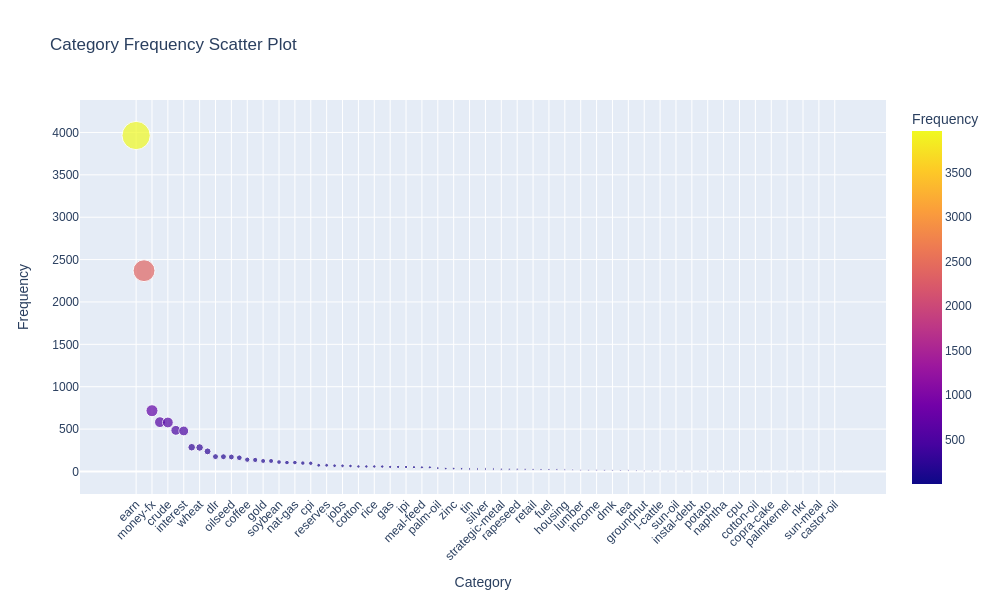
\includegraphics[width=1\textwidth]{reuter4.png} 
  \caption{Caption for your image}
  \label{fig:your-label}
\end{figure}
\begin{figure}[h!]
  \centering
  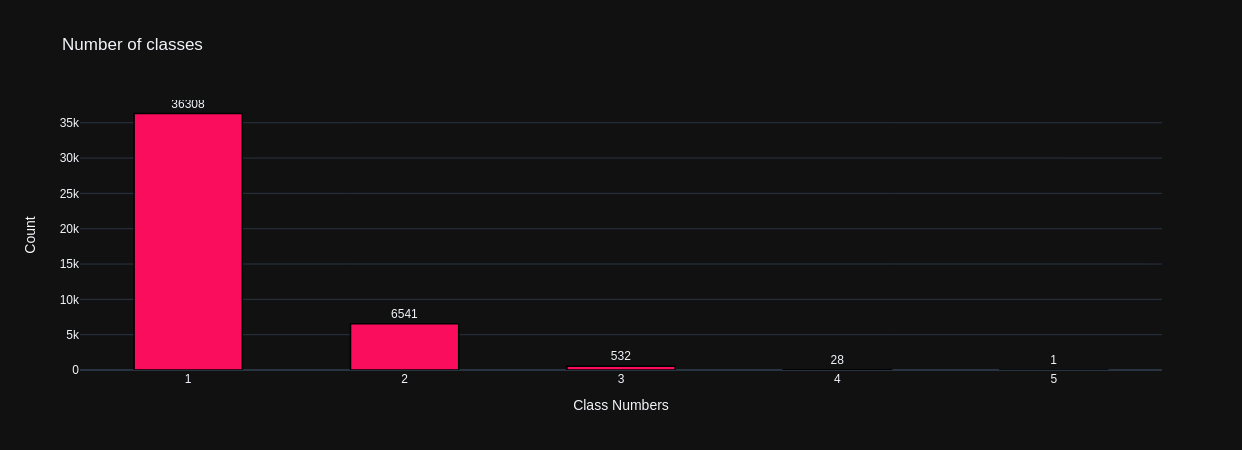
\includegraphics[width=1\textwidth]{goemo1.png} 
  \caption{Caption for your image}
  \label{fig:your-label}
\end{figure}
\begin{figure}[h!]
  \centering
  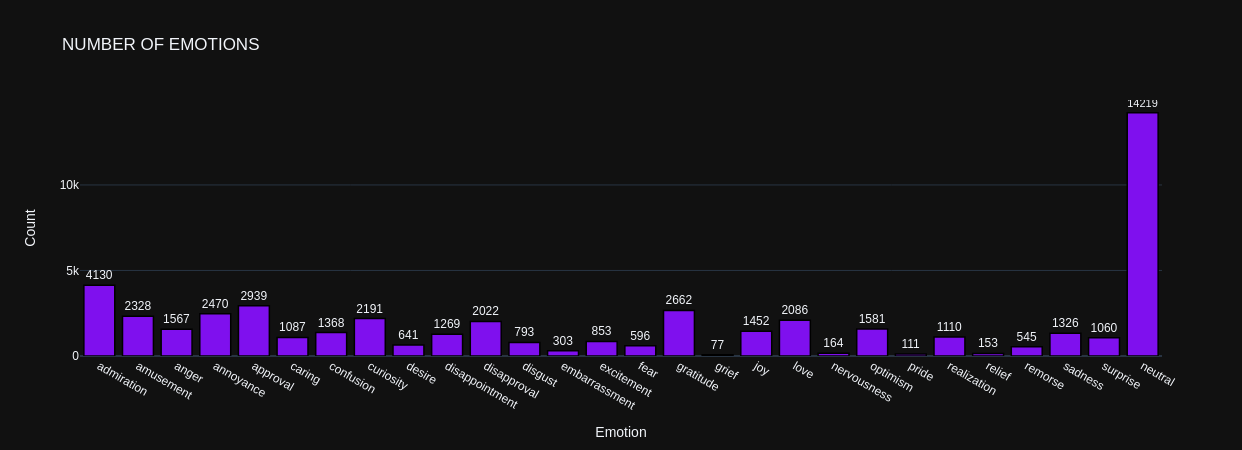
\includegraphics[width=1\textwidth]{goemo2.png} 
  \caption{Caption for your image}
  \label{fig:your-label}
\end{figure}
\begin{figure}[h!]
  \centering
  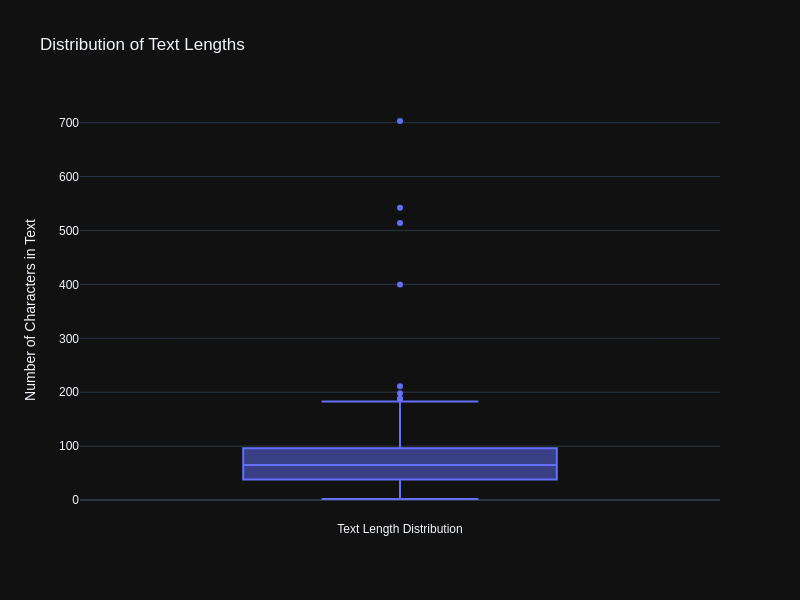
\includegraphics[width=1\textwidth]{goemo3.png} 
  \caption{Caption for your image}
  \label{fig:your-label}
\end{figure}
\FloatBarrier
\section{Gradio App User Interface}\label{sec:demo_ui}
\begin{figure}[h!]
  \centering
  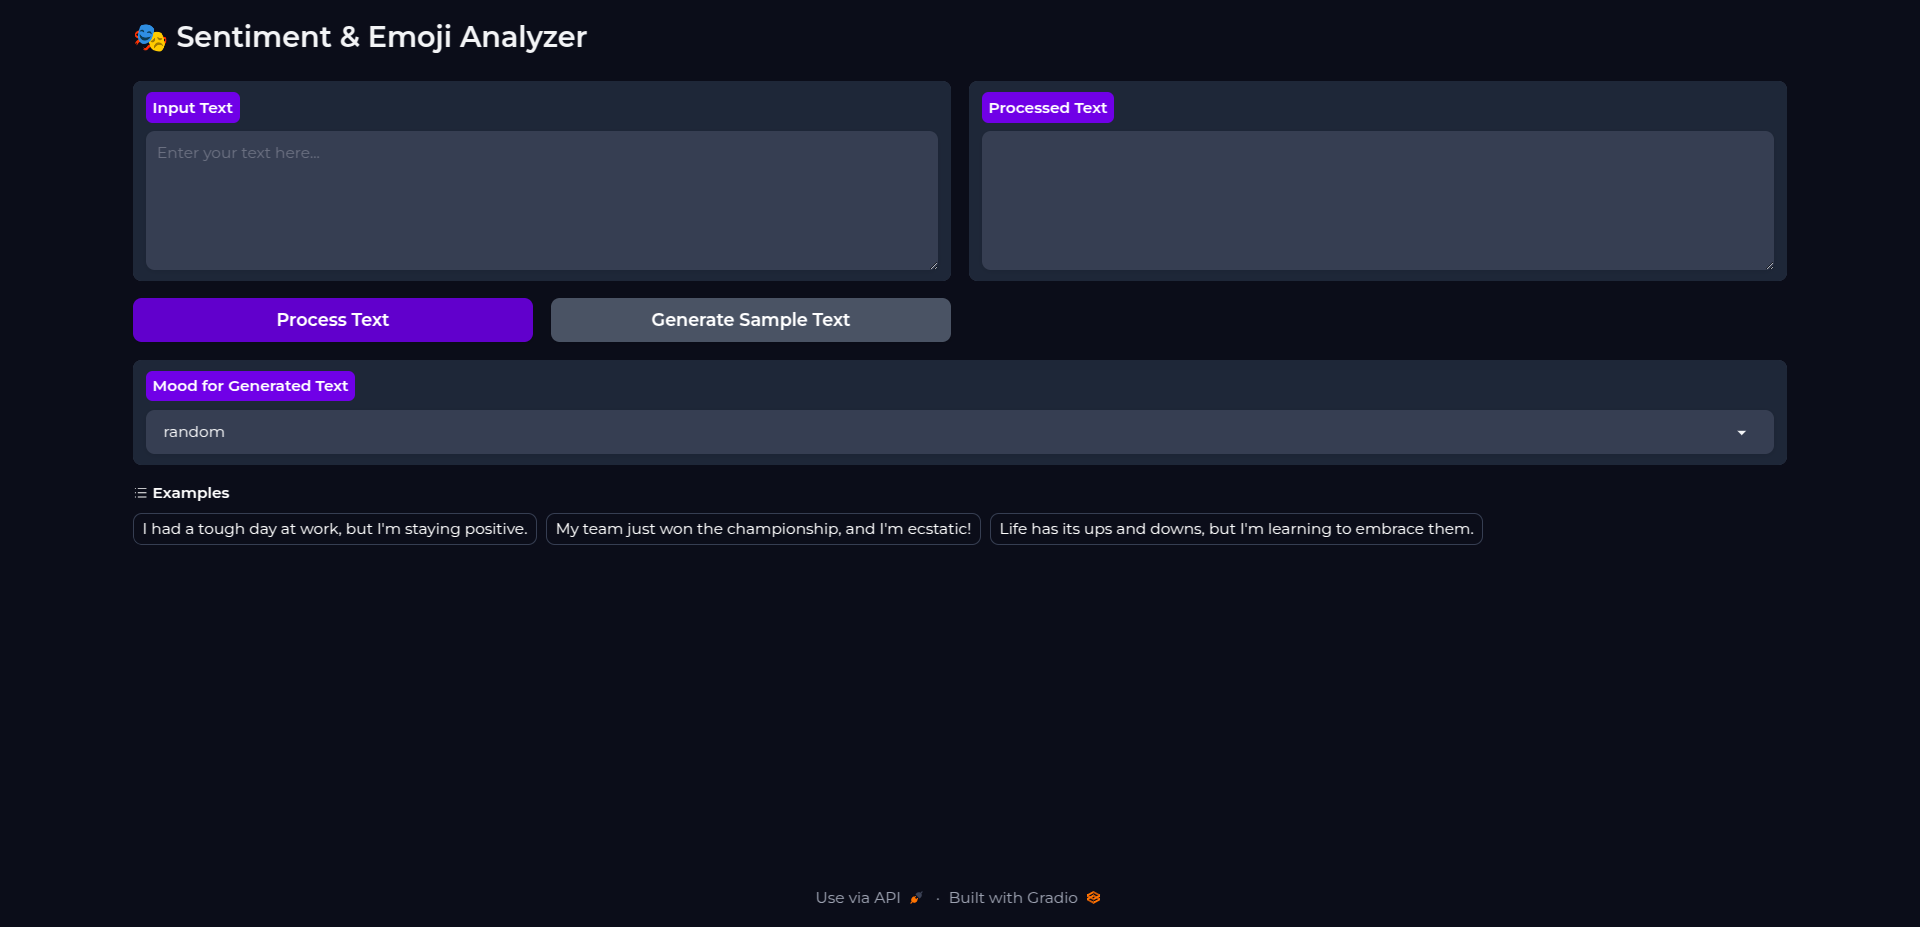
\includegraphics[width=1\textwidth]{demo.png} 
  \caption{Gradio demo}
  \label{fig:your-label}
\end{figure}
\begin{figure}[h!]
  \centering
  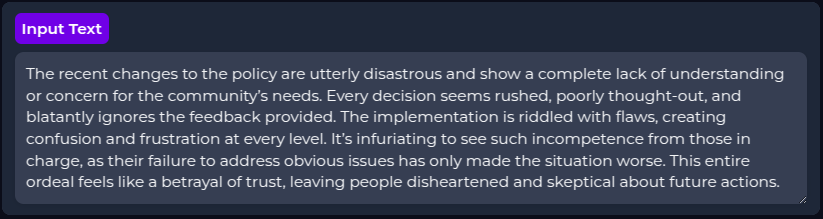
\includegraphics[width=1\textwidth]{demo_input.png} 
  \caption{Gradio input}
  \label{fig:your-label}
\end{figure}
\begin{figure}[h!]
  \centering
  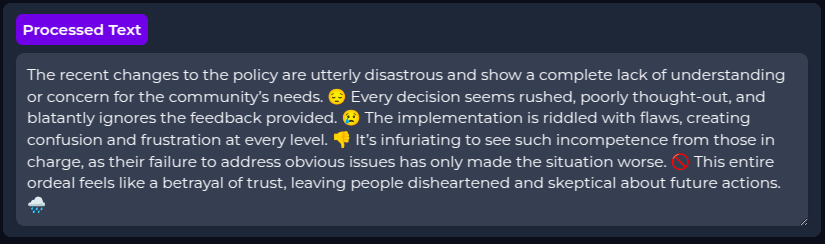
\includegraphics[width=1\textwidth]{demo_output.png} 
  \caption{Gradio outpu}
  \label{fig:your-label}
\end{figure}
\end{document}
